\section{Resultados}

% CONVERGENCIA DEL MÉTODO
\subsection{Experimento de la convergencia del método}
\begin{figure}[H]{}
\centering
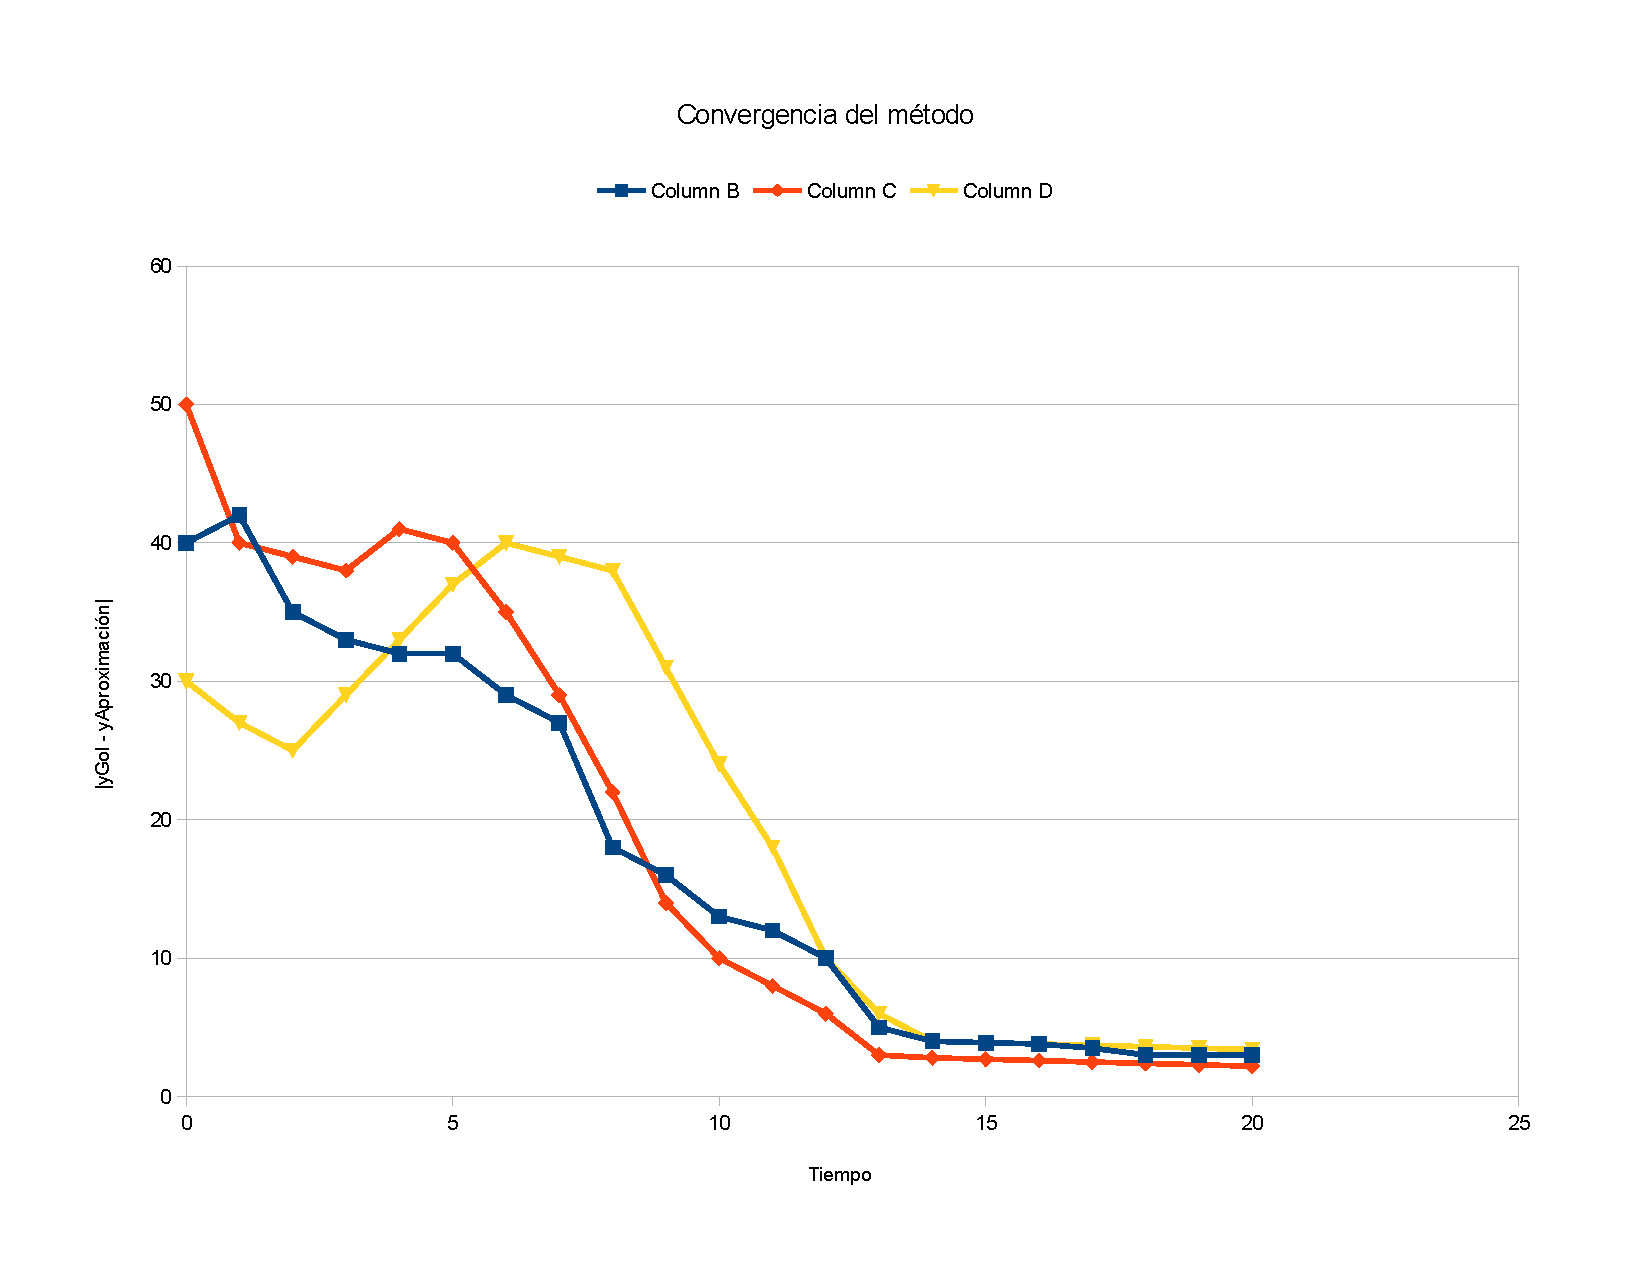
\includegraphics[scale=0.5]{graphs/convergenciaMetodo.pdf}
\label{convergenciaMetodo}
\end{figure}

Azul: rectas. Amarillo: cuadráticas. Naranja: cúbicas.

% TASA DE EFICIENCIA EN FUNCIÓN DE LA CANTIDAD DE SUJETOS CONSIDERADOS
\subsection{Experimento de tasa de efectividad en función del grado}
\begin{figure}[H]{}
\centering
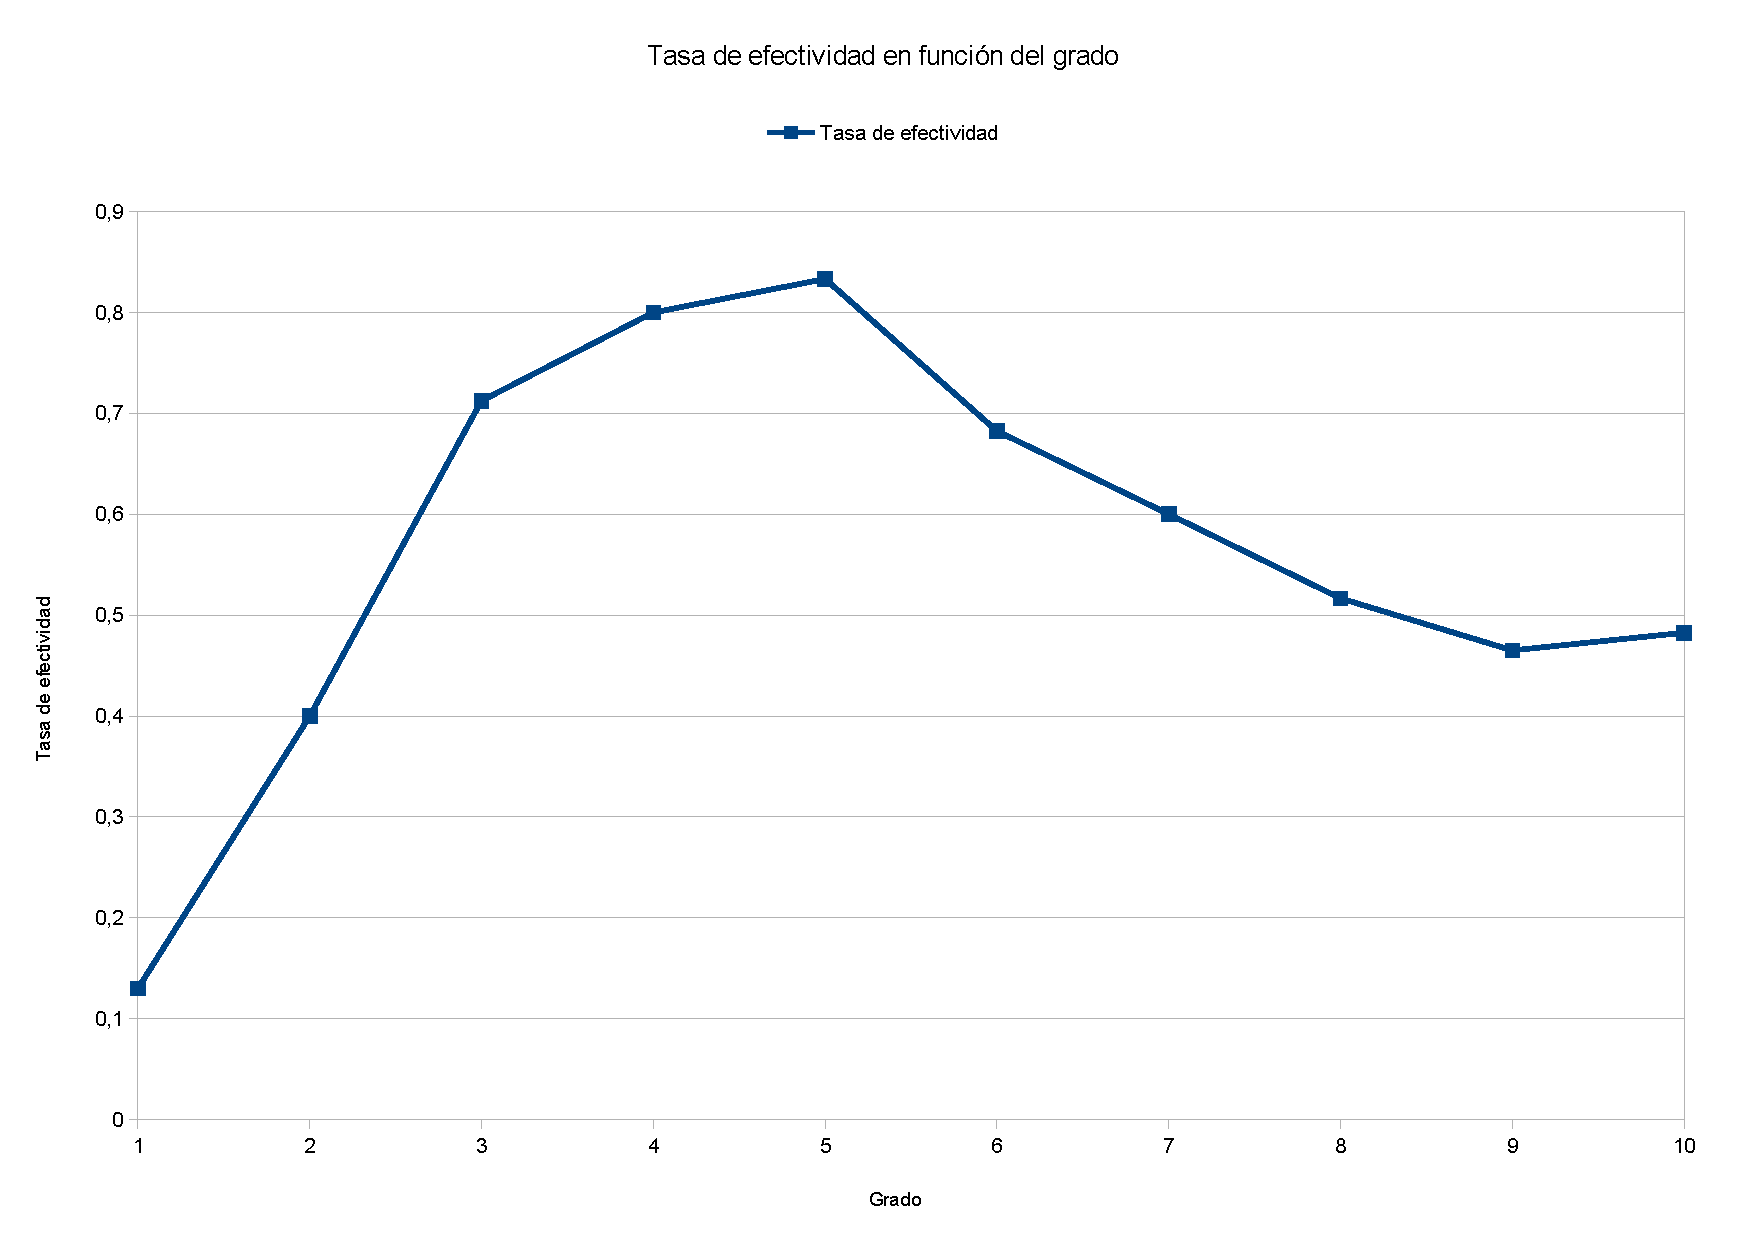
\includegraphics[scale=0.5]{graphs/TEvsGrado.pdf}
\label{TEvsGrado}
\end{figure}

% TASA DE EFICIENCIA EN FUNCIÓN DE LA CANTIDAD DE COMPONENTES PRINCIPALES TOMADAS
\subsection{Experimento de tasa de efectividad en función de los puntos considerados}
\begin{figure}[H]{}
\centering
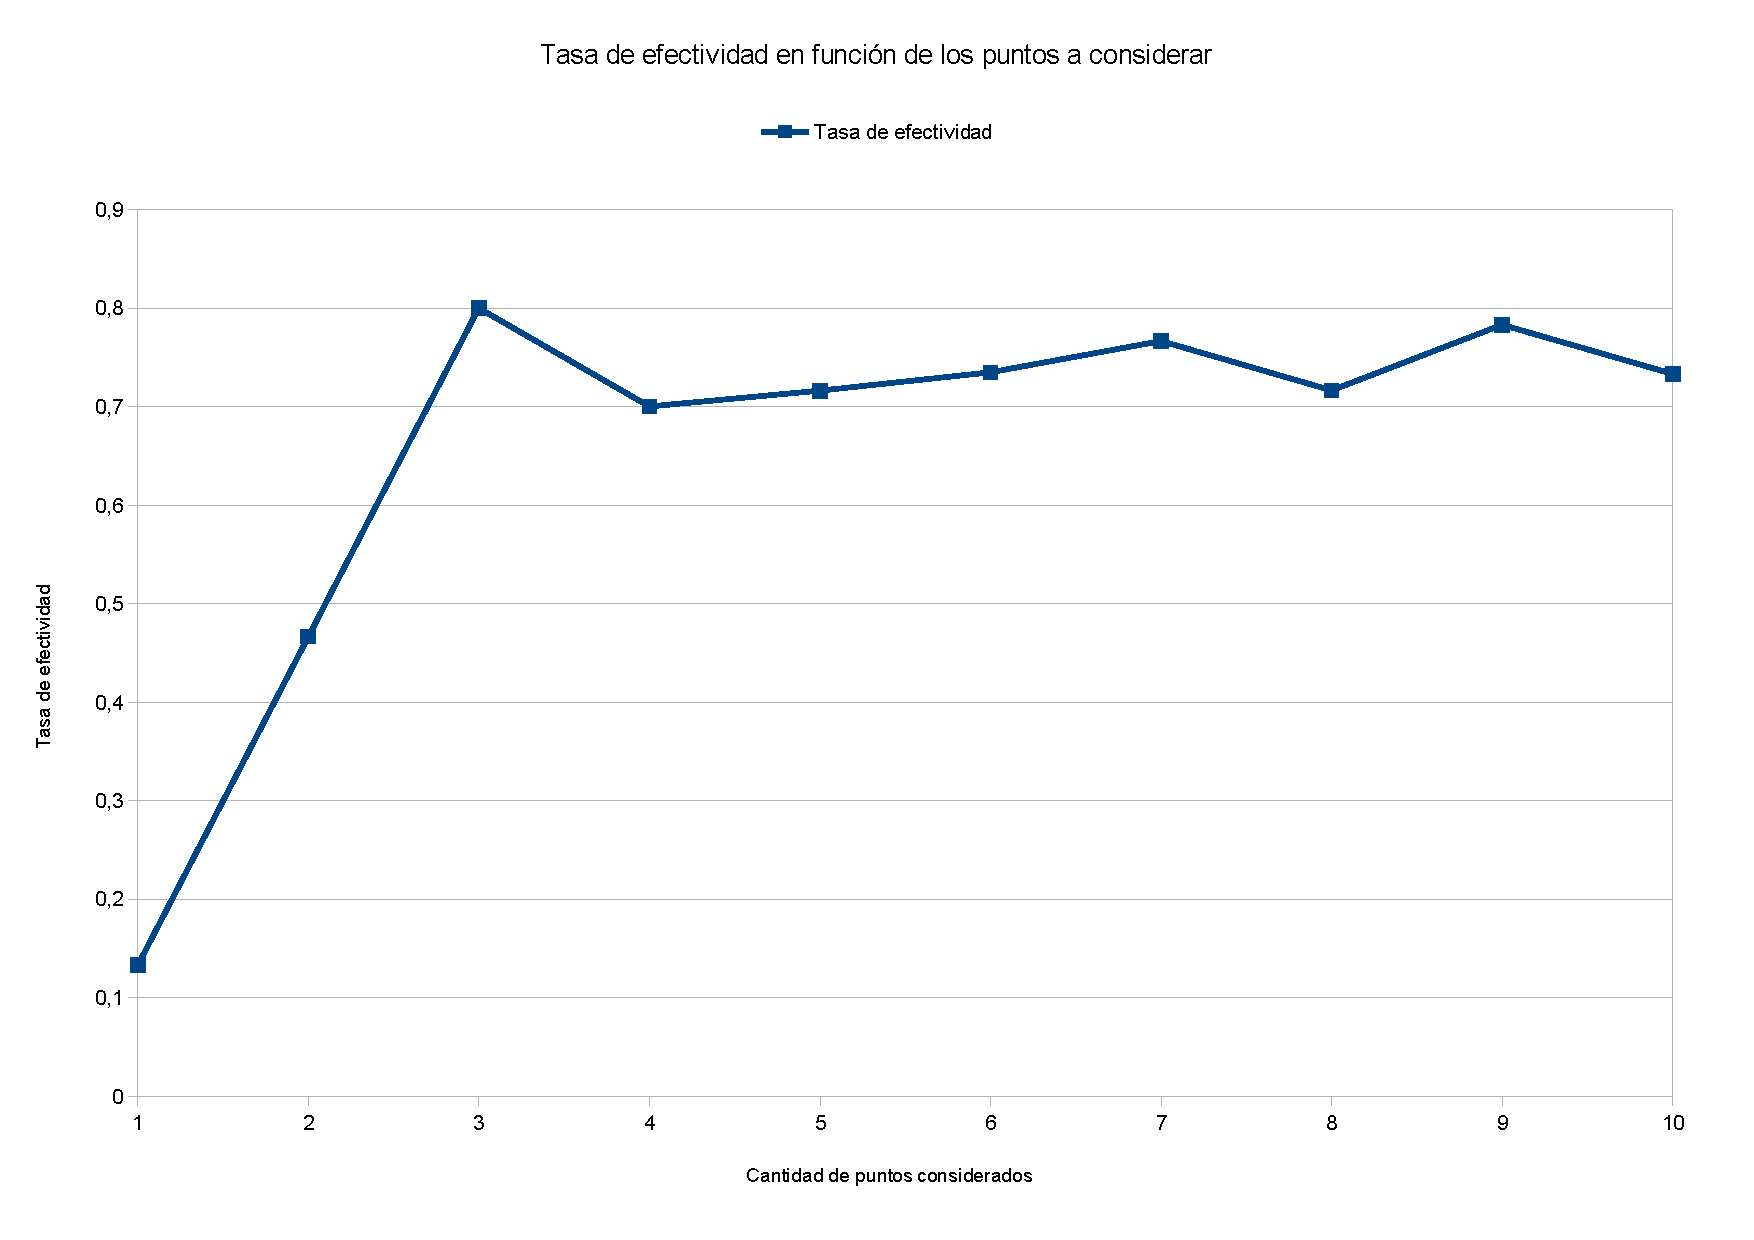
\includegraphics[scale=0.5]{graphs/TEvsMediciones.pdf}
\label{TEvsPac}
\end{figure}
